\Cref{sec:photon_selection} introduced the best-photon candidate strategy, 
as well as selection to suppress events 
where the photon is misidentified or originates in sources different than \BtoXsgamma.
However, as was seen before in, for example. \Cref{fig:photon_reco_candidates_bplus,fig:photon_reco_candidates_bzero},
\epem\ra\qqbar events provide the vast majority of photon candidates.
Therefore, a dedicated event-selection for this type of background was devised.
It takes advantage of  different event topologies expected for $\FourS\to\qqbar$ and $\epem\ra\qqbar$ events.
Loosely speaking, events where a $\FourS\to\BB$ decay is present tend to be more `spherical', when compared with $\epem\ra\qqbar$ events that exhibit a `jet-like' distribution.
This is related to the fact that \epem collissions at $B$ dactory experiments have just enough energy to produce a $B$ pair almost at rest, which means that its decays products, on average, tend to be distributed uniformly in polar and azimuthal angle.
On the other hand, light-quark pairs, produced in \epem collision events, also gain a substantial amount of back-to-back momentum which tends to spread their decay products. 
The schematic idea of this is shown in \Cref{fig:continuum_schematic}.
This section will provide an in-depth discussion on how the discrimination between \BtoXsgamma and continuum is achieved using a \BDT.

\begin{figure}[htbp!]
    \centering
    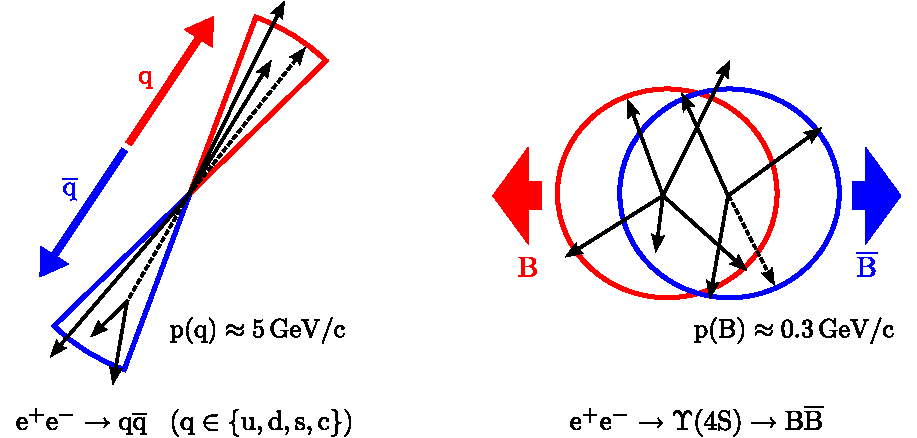
\includegraphics[width=0.6\textwidth]{figures/continuum_suppression/figure_continuum_suppression_event_shapes.pdf}
    \caption{\label{fig:continuum_schematic} Schematic illustration of continuum and \BB events created after an \epem collision in $B$ factories.
    Events where a $B$ meson is produced are generally more spherical, due to the fact that \FourS is produced at rest and its decays products tend to not have a preferred direction.
    Typical momenta of light-quark and \BB mesons are shown.
    The specific directions shown are illustrative only. 
    }
\end{figure}

\subsection{Training event pre-selection}\label{sec:preselection}

Before a \BDT is trained, it is generally desirable to prepare the datasets such that the classifier 
is able to learn based on relevant data.
Such data preprocessing will be performed based on variables described in \Cref{sec:photon_selection}.
The classifier will then be trained on the reduced dataset

In order to find optimal selections, a figure-of-merit study is performed for each observable.
Two figure of merit options were considered for this analysis, a more standard figure-of-merit $\mathrm{FOM}_1$:
\begin{equation}\label{eq:soversqrtsplusb}
    \mathrm{FOM}_1 = \frac{\mathsf{S}}{\sqrt{\mathsf{S}+\mathsf{B}}},
\end{equation}
and $\mathrm{FOM}_2$ defined in Ref.\cite{Punzi:2003bu} (often referred to as `Punzi' figure-of-merit):
\begin{equation}\label{eq:punzi_fom}
    \mathrm{FOM}_2 = \frac{\mathsf{S}}{\mathsf{S}_0} \frac{1}{\frac{3}{2}+\sqrt{\mathsf{B}}}.
\end{equation}
In both equations, $\mathsf{S}$ is the number of signal events after selection, 
$\mathsf{B}$ is the number of background events after selection, 
and $\mathsf{S}_0$ is the number of signal events before selection.
Although \Cref{eq:punzi_fom} was derived with search-like analyses in mind, 
it is utilised in this analysis to minimise signal model dependancy: the ratio $\mathsf{S}/\mathsf{S}_0$ present in the definition reduces out many model-dependant effects.

For each figure of merit calculation, background events ($\mathsf{B}$) are calculated based on generic \MC,
whereas signal events, $\mathsf{S}$, are calculated based on signal \MC, to ensure a high statistics sample.
In the case of \Cref{eq:soversqrtsplusb}, an appropriate scaling for $\mathsf{S}$ is also used.
Each dataset has duplicate tag-candidate events randomly removed, by picking a random tag-side candidate.
Each figure of merit is then calculated for 200 equally spaced selections in the target observable.
The maximum figure-of-merit point is taken as the optimal pre-selection for each of the variables.
This procedure is shown for $\mathrm{FOM}_2$ in \Cref{fig:selection_optimisations}.
Results for $\mathrm{FOM}_1$ are used as a cross-check for $\mathrm{FOM_2}$ but turn out to be consistent.
Equivalent procedure for $\mathrm{FOM}_1$ is shown in \Cref{sec:appendix_sqrtsplusb_optimisation}.
The resulting optimal selections are also shown in the Figures.

\begin{figure}[htbp!]
    \centering
    \subcaptionbox{\label{fig:bp_zmva_optimisation}}{
            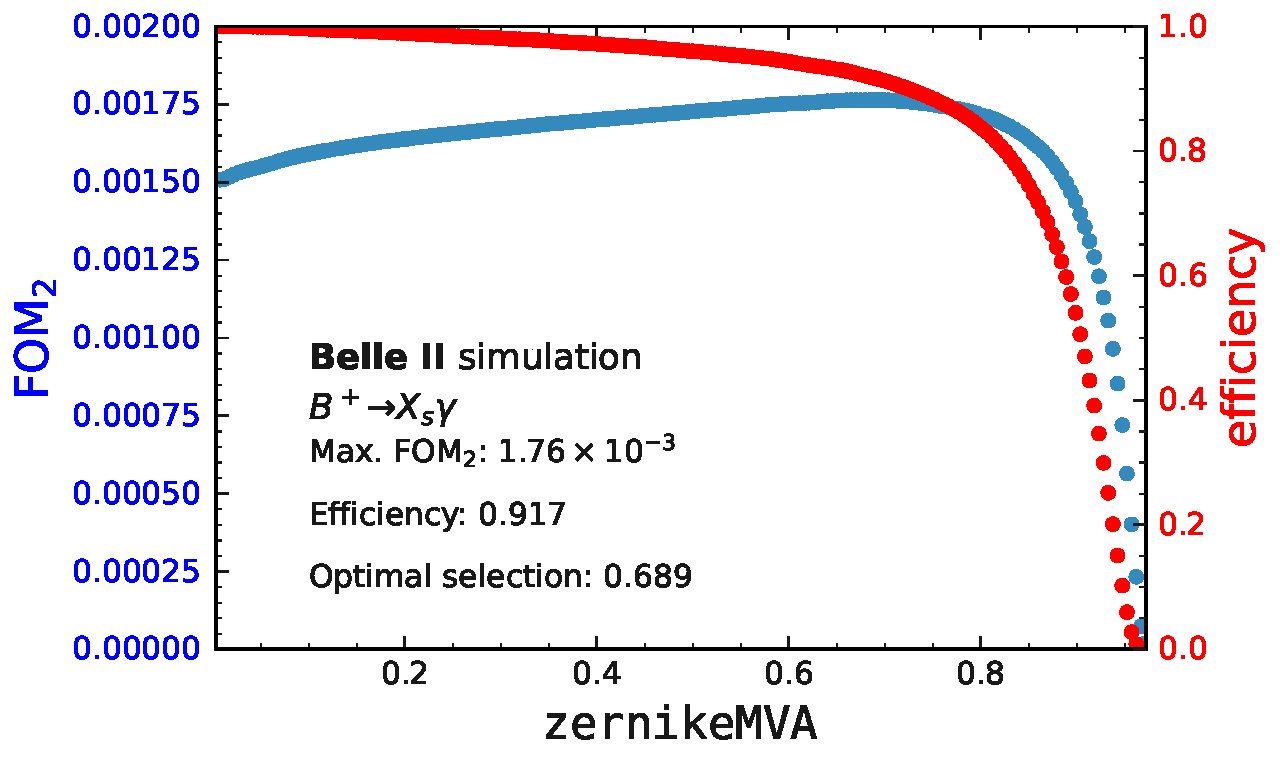
\includegraphics[width=0.3\textwidth]{figures/continuum_suppression/Bp_zernikeMVA_optimisation_punzi.pdf}
        }
    \subcaptionbox{\label{fig:bp_piveto_optimisation}}{
            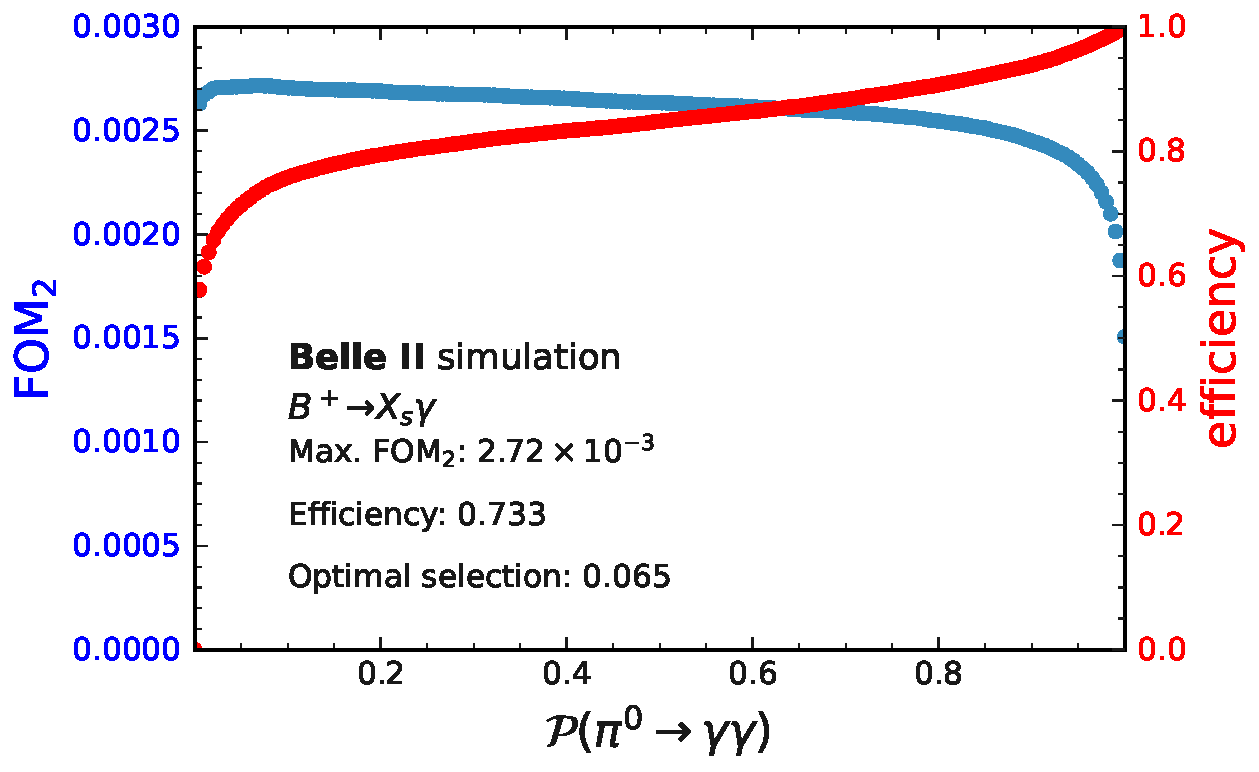
\includegraphics[width=0.3\textwidth]{figures/continuum_suppression/Bp_piVeto_optimisation_punzi.pdf}
        }
    \subcaptionbox{\label{fig:bp_etaveto_optimisation}}{
            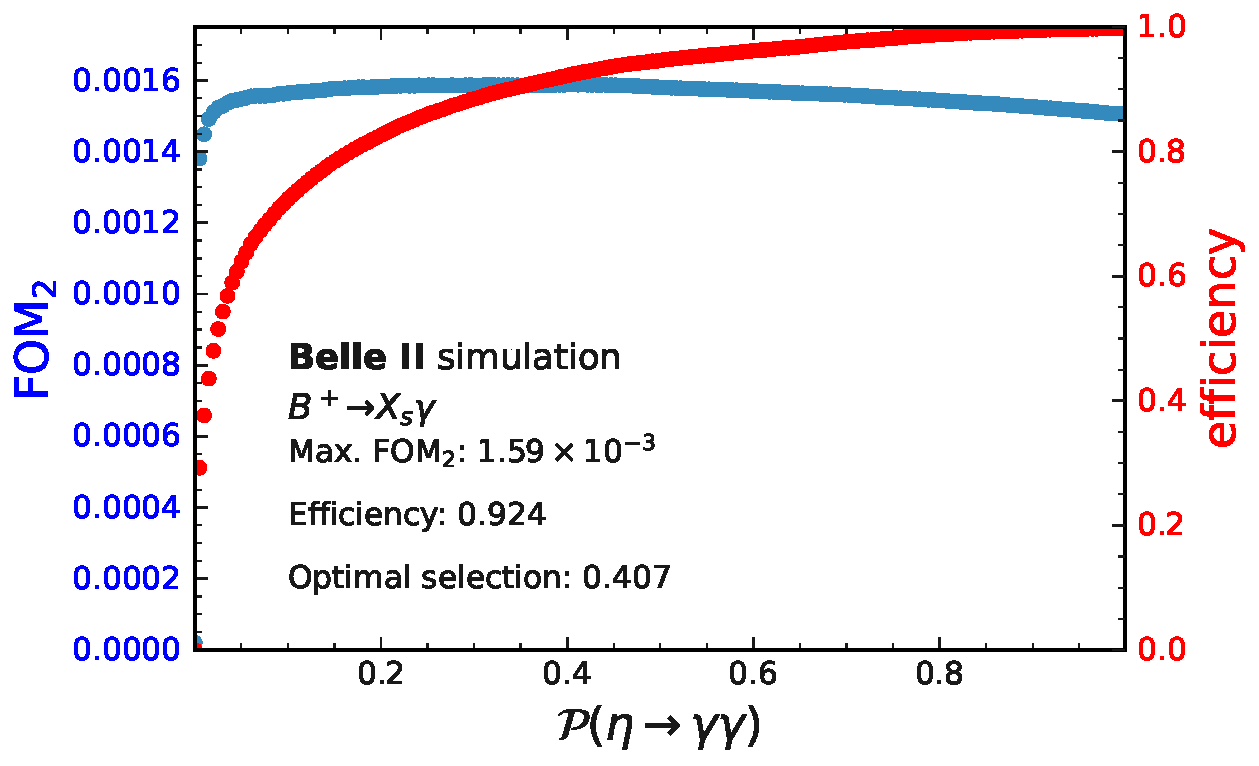
\includegraphics[width=0.3\textwidth]{figures/continuum_suppression/Bp_etaVeto_optimisation_punzi.pdf}
        }
    \subcaptionbox{\label{fig:bz_zmva_optimisation}}{
            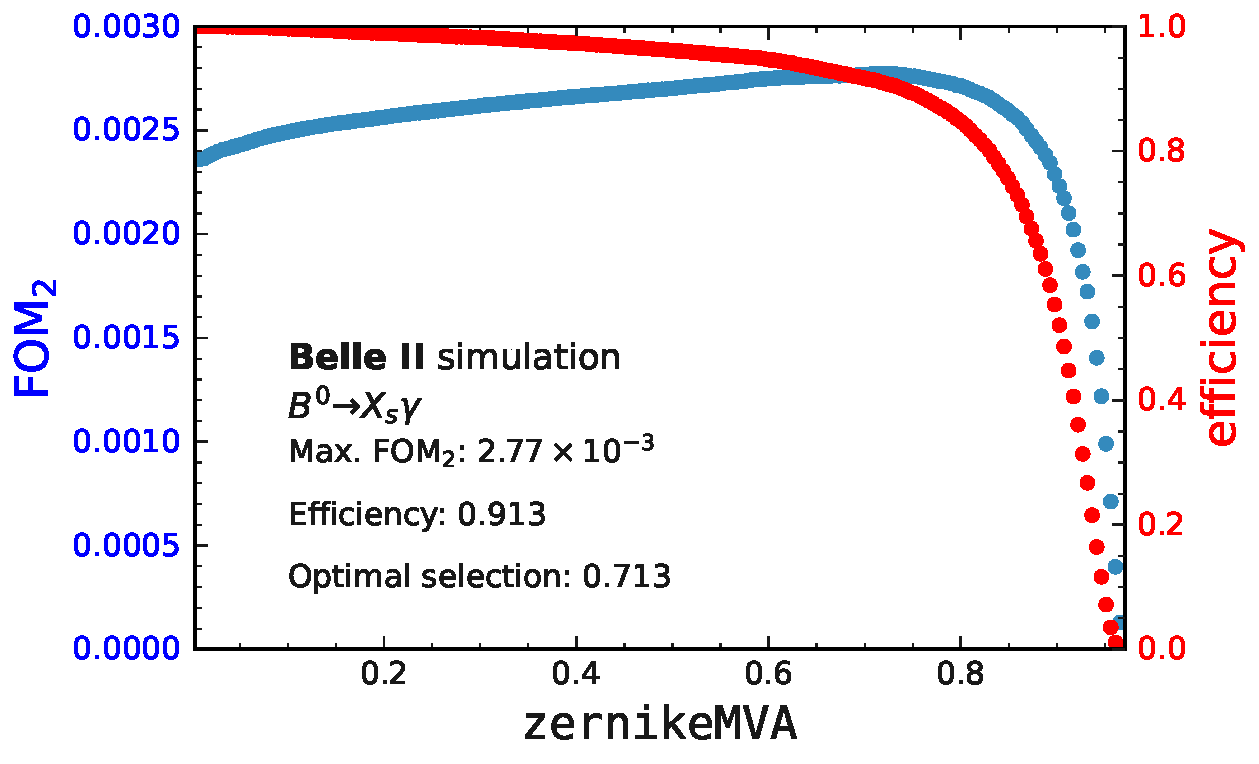
\includegraphics[width=0.3\textwidth]{figures/continuum_suppression/Bz_zernikeMVA_optimisation_punzi.pdf}
        }
    \subcaptionbox{\label{fig:bz_piveto_optimisation}}{
            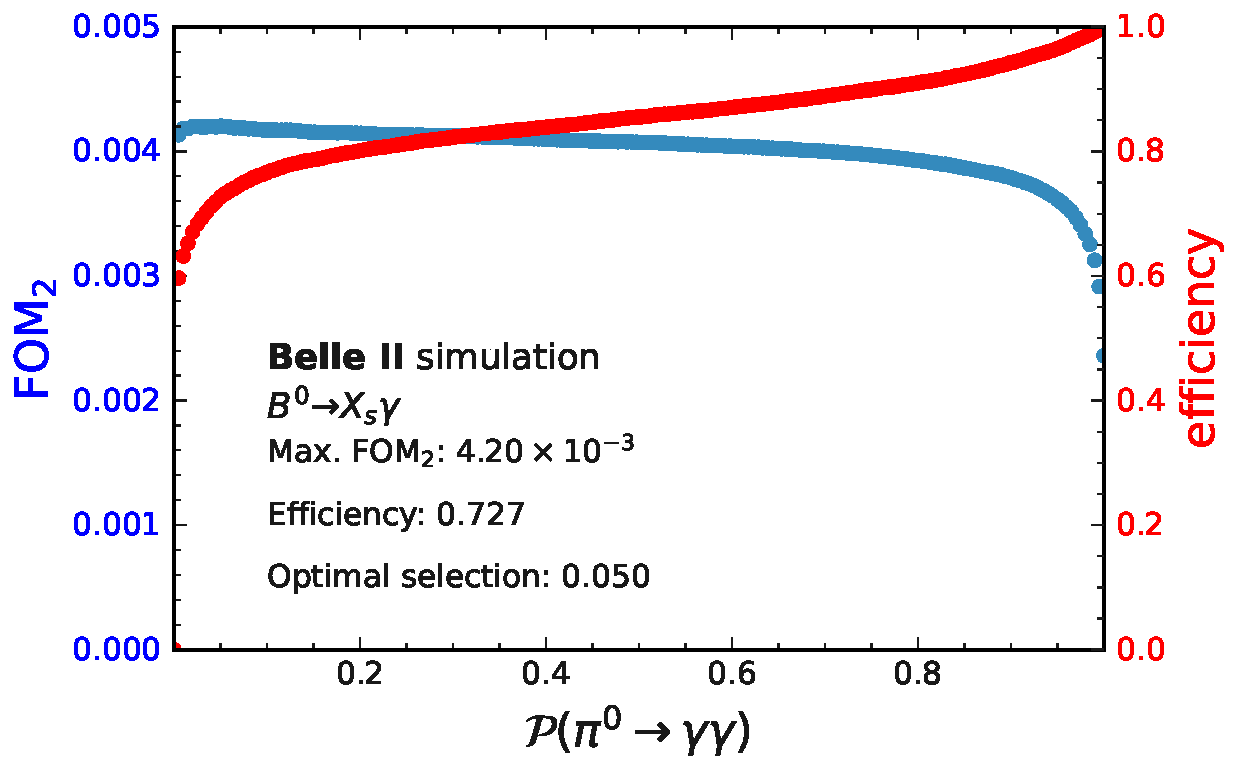
\includegraphics[width=0.3\textwidth]{figures/continuum_suppression/Bz_piVeto_optimisation_punzi.pdf}
        }
    \subcaptionbox{\label{fig:bz_etaveto_optimisation}}{
            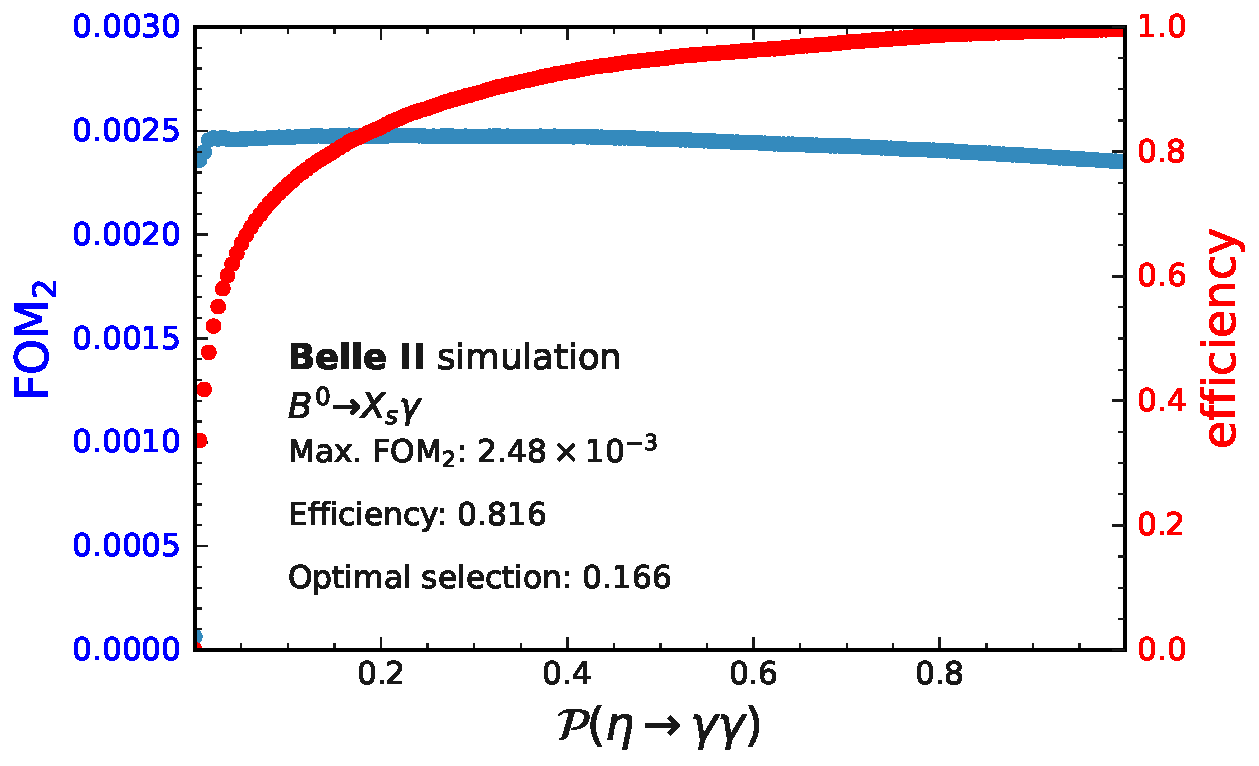
\includegraphics[width=0.3\textwidth]{figures/continuum_suppression/Bz_etaVeto_optimisation_punzi.pdf}
        }
    \caption{\label{fig:selection_optimisations} Optimal selection calculation for observables
    described in \Cref{sec:photon_selection} based on $\mathrm{FOM}_2$ (see \Cref{eq:punzi_fom}).
    For \BptoXsgamma events the tests are shown
    in \Cref{fig:bp_zmva_optimisation,fig:bp_piveto_optimisation,fig:bp_etaveto_optimisation},
    and for \BztoXsgamma in \Cref{fig:bz_zmva_optimisation,fig:bz_piveto_optimisation,fig:bz_etaveto_optimisation}.
    The figures show efficiency and $\mathrm{FOM}_2$ score calculated for 200 selections of \piVeto, \etaVeto and \ZMVA.
    The maximum value of $\mathrm{FOM}_2$, the corresponding selection and efficiency are shown as well.
    }
\end{figure}

The results between \Bp and \Bz modes, as well as using $\mathrm{FOM}_1$ and $\mathrm{FOM}_2$ are consistent, with only marginal differences.
Therefore, due to the model-independance of $\mathrm{FOM}_2$, this figure-of-merit will be the only one discussed henceforth.
At this stage, it is unnecessary to choose the `best' selection, as another simultaneous optimisation will be performed later, together with continuum suppression \BDT output.
\todo[inline]{(see XXX when I optimise)}. 
The main goal is to reduce the sample size to include only relevant data, such that the trained \BDT can make decisions for difficult cases that are not easily distinguishable using simple selection.
Based on \Cref{fig:selection_optimisations}, pre-selections are chosen, which suppress background but retain most of the signal.
The requirement for a loose selection are tailored such that more than 75\% of \BtoXsgamma candidates are retained and are shown in \Cref{tab:preselections}.

\begin{table}[htbp!]
    \centering
    \caption{\label{tab:preselections} \todo[inline]{add caption}}
    
    \begin{tabular}{|lr|}
    \hline
    Variable &    Loose selections \\
    \hline
    \ZMVA & $>0.5$ \\
    \piVeto            & $<0.4$ \\
    \etaVeto           & $<0.4$ \\
    
    \hline
    
    $B^+$ mode: $\gamma$ candidate retention efficiency & 75.4\% \\
    $B^0$ mode: $\gamma$ candidate retention efficiency & 76.7\% \\
    \hline
    \end{tabular}

\end{table}

\subsection{Continuum suppression observables}\label{sec:continuum_features}

